The rhythm patterns are computed using a spectral flux\index{Spectral flux} feature (called LogFilt- SpecFlux as proposed by \citeA{bock:12:onseteval} and used further by \citeA{krebs:13:bpm}) that is used for detecting musical onsets in audio recordings. The \gls{STFT} of the audio signal with a window size of 46.4 ms (2047 samples of audio at a sampling rate of 44.1 kHz), DFT size of 2048 and hop size of 20 ms is computed from audio. The successive difference between frames of the logarithm of the filter bank energies in 82 different bands is then computed. Since the bass onsets have significant information about the rhythmic patterns, the features are computed in two frequency bands (Low: $\leq$ 250 Hz, High: $>$ 250 Hz) to additionally consider the bass onsets. The process of computing the spectral flux feature is outlined in \figref{fig:obs:featcomp}. 

Using beat and downbeat annotated training data, the audio features from all music pieces in a specific \gls{tala} are then grouped into cycle length sequences, and interpolated to equal lengths using a fine grid. A mean of all such cycle length sequence instances for a specific \gls{tala} is computed in both the frequency bands and used as a representative rhythmic pattern illustrated here. 

At the outset, it is necessary to note here that the patterns played in a \gls{tala} cycle are to be described using timing, energy and timbre descriptors. The rhythm patterns generated here using the spectral flux feature and can only explain timing and energy accents. A minor effect of timbre can be seen in these rhythm patterns, but are predominantly affected by the other two characteristics. These patterns are averaged over the whole dataset for a \gls{tala}, and hence cannot capture specific nuances of individual pieces, but only can give a broad perspective. The patterns here are indicative of the surface rhythm present in the audio recordings, and hence completely reflect the underlying canonical metrical structures. % List down other limitations of this approach. 

\figrefs{fig:tt:CMDf:adi}{fig:tt:CMD:khandaChapu}\ show the ensemble average of cycle length patterns over all the pieces in the dataset for each \gls{tala}, computed using the spectral flux feature in two different frequency bands as outlined above. In each figure, the bottom pane corresponds to the low frequency band ($\protect\obsLow$) and the top pane corresponds to the high frequency band ($\protect\obsHigh$). The abscissa is the beat number within the cycle (dotted lines), with 1 indicating the \gls{sama} (marked with a red line). The start of each \gls{anga} is indicated with beat numbers at the top of each pane (\gls{sama} shown as $\times$). The patterns in each figure pane is normalized so that maximum value is 1, to comment on relative onset strengths at different metrical positions of the cycle. 

The rhythm patterns are roughly indicative of the energies of mridangam strokes played in the cycle. In the figures, the bottom pane that shows the low frequency band has content from the left bass drum while the top pane has content predominantly from the right pitched drum (and additionally from the lead melody). Hence, for the purpose of this discussion, we use the terms left and right accents to refer to the accents in rhythm patterns shown on the bottom and top pane, respectively. The left and right accents provide interesting insights into the patterns played within a \gls{tala} cycle. In addition, these rhythm patterns help in meter tracking. 
% Tala pattern: CMDf-adi-all-lo230-superflux-mvavg-normZ, CMDf-adi-all-hi250-superflux-mvavg-normZ
\begin{figure}[t]
\captionsetup[subfigure]{labelformat=empty}
\centering
\subfloat[]{\label{fig:tt:CMDf:adi:hi}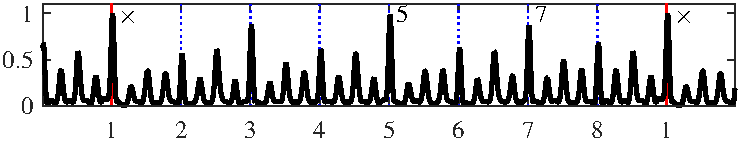
\includegraphics[width=\textwidth]{talaPatts/CMDf-adi-all-hi250-superflux-mvavg-normZ.pdf}} \\ \vspace{-1.35cm}
\subfloat[]{\label{fig:tt:CMDf:adi:lo}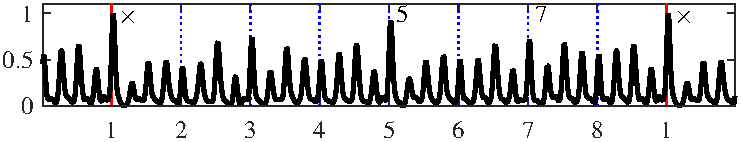
\includegraphics[width=\textwidth]{talaPatts/CMDf-adi-all-lo230-superflux-mvavg-normZ.pdf}}
\caption[Rhythm patterns in \gls{adi} \gls{tala} learned from \acrshort{CMDf} dataset]{Cycle length rhythmic patterns learned from \acrshort{CMDf} dataset for \gls{adi} \gls{tala}. In each of the following \protect\figrefs{fig:tt:CMDf:adi}{fig:tt:CMD:khandaChapu}, the patterns are computed from spectral flux feature and averaged over all the pieces in the dataset. The bottom/top pane corresponds to the low/high frequency bands, respectively. The abscissa is the beat number within the cycle (dotted lines), with 1 indicating the \gls{sama} (marked with a red line). The start of each \gls{anga} is indicated with beat numbers at the top of each pane (\gls{sama} shown as $\times$). The plot shows the cycle extended by a beat at the beginning and end to illustrate the cyclic nature of the \gls{tala}.}\label{fig:tt:CMDf:adi} %CMDf-adi-all-hi250-superflux-mvavg-normZ,CMDf-adi-all-lo230-superflux-mvavg-normZ
\end{figure}
%
% Tala pattern: CMD-adi-all-lo230-superflux-mvavg-normZ, CMD-adi-all-hi250-superflux-mvavg-normZ
\begin{figure}
\captionsetup[subfigure]{labelformat=empty}
\centering
\subfloat[]{\label{fig:tt:CMD:adi:hi}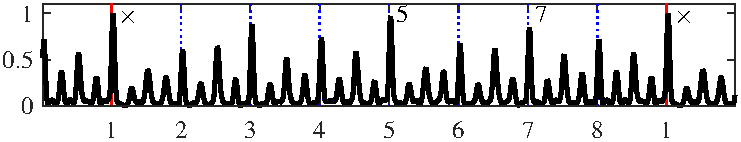
\includegraphics[width=\textwidth]{talaPatts/CMD-adi-all-hi250-superflux-mvavg-normZ.pdf}} \\ \vspace{-1.35cm}
\subfloat[]{\label{fig:tt:CMD:adi:lo}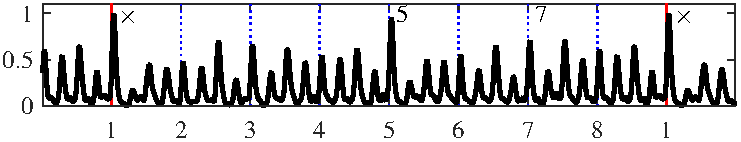
\includegraphics[width=\textwidth]{talaPatts/CMD-adi-all-lo230-superflux-mvavg-normZ.pdf}}
\caption[Rhythm patterns in \gls{adi} \gls{tala} learned from \acrshort{CMDs} dataset]{Cycle length rhythmic patterns learned from \acrshort{CMDs} dataset for \gls{adi} \gls{tala}.}\label{fig:tt:CMD:adi}
\end{figure}

We list down and discuss some salient qualitative observations from figures for each \gls{tala}, for both \acrshort{CMDf} dataset and its subset \acrshort{CMDs}. The \figrefs{fig:tt:CMDf:adi}{fig:tt:CMD:khandaChapu}\ show the cycle length rhythm patterns for all \glspl{tala} for both \acrshort{CMDf} and \acrshort{CMDs} datasets. For each \gls{tala}, we plot the rhythm patterns together to compare patterns across the short excerpts in \acrshort{CMDs} dataset and full length pieces in \acrshort{CMDf} dataset. 

Overall, we see stronger accents on the \glspl{akshara}, with \gls{sama} having the strongest accent in most cases. We can clearly see the accents organized in three different strengths, reflecting the metrical levels of the \gls{anga}, the beat and the \gls{akshara}. The two \gls{akshara} long beats in \gls{mishra chapu} and \gls{khanda chapu} \glspl{tala}, and the four \gls{akshara} long beats in \gls{adi} and \gls{rupaka} \glspl{tala} can be additionally seen. The patterns and \glspl{theka} played in Carnatic music are quite diverse, and no obvious representative \gls{tala} pattern can be inferred, apart from the varied accents at three metrical levels. 
% Tala pattern: CMDf-rupaka-all-lo230-superflux-mvavg-normZ, CMDf-rupaka-all-hi250-superflux-mvavg-normZ
\begin{figure}[t]
\captionsetup[subfigure]{labelformat=empty}
\centering
\subfloat[]{\label{fig:tt:CMDf:rupaka:hi}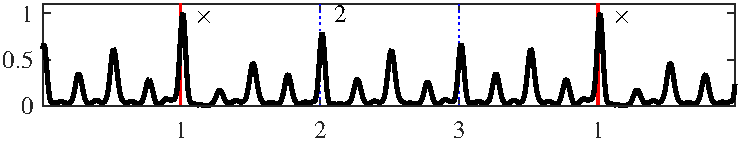
\includegraphics[width=\textwidth]{talaPatts/CMDf-rupaka-all-hi250-superflux-mvavg-normZ.pdf}} \\ \vspace{-1.35cm}
\subfloat[]{\label{fig:tt:CMDf:rupaka:lo}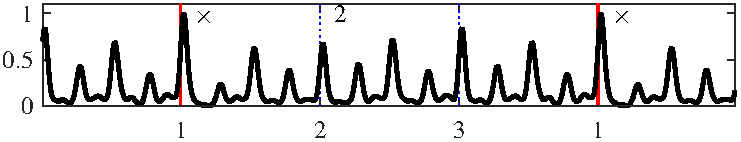
\includegraphics[width=\textwidth]{talaPatts/CMDf-rupaka-all-lo230-superflux-mvavg-normZ.pdf}}
\caption[Rhythm patterns in \gls{rupaka} \gls{tala} learned from \acrshort{CMDf} dataset]{Cycle length rhythmic patterns learned from \acrshort{CMDf} dataset for \gls{rupaka} \gls{tala}.}\label{fig:tt:CMDf:rupaka}
\end{figure}
%
% Tala pattern: CMD-rupaka-all-lo230-superflux-mvavg-normZ, CMD-rupaka-all-hi250-superflux-mvavg-normZ
\begin{figure}[t]
\captionsetup[subfigure]{labelformat=empty}
\centering
\subfloat[]{\label{fig:tt:CMD:rupaka:hi}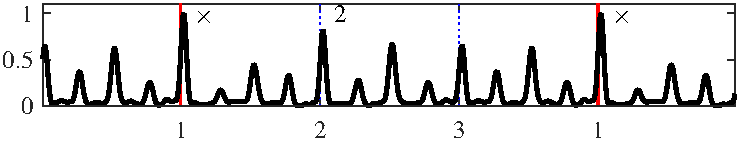
\includegraphics[width=\textwidth]{talaPatts/CMD-rupaka-all-hi250-superflux-mvavg-normZ.pdf}} \\ \vspace{-1.35cm}
\subfloat[]{\label{fig:tt:CMD:rupaka:lo}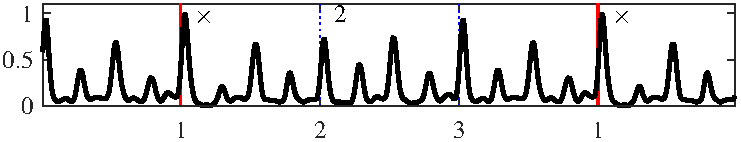
\includegraphics[width=\textwidth]{talaPatts/CMD-rupaka-all-lo230-superflux-mvavg-normZ.pdf}}
\caption[Rhythm patterns in \gls{rupaka} \gls{tala} learned from \acrshort{CMDs} dataset]{Cycle length rhythmic patterns learned from \acrshort{CMDs} dataset for \gls{rupaka} \gls{tala}.}\label{fig:tt:CMD:rupaka}
\end{figure}
%

The patterns illustrated here are average patterns that occur and do not tell us much about the various individual patterns that might occur in specific points in particular recordings. The \glspl{tala} are metrical structures that allow many different patterns to be played, and not a specific rhythm. It is further seen that the first \gls{akshara} after \gls{sama} has softer accents. Fewer strokes are played after the \gls{sama}, to emphasize that the \gls{sama} has just passed and a new cycle has begun. It might also perhaps indicate some form of recovery time after the intense stroke-playing towards the end of the cycle. 

The rhythm patterns computed using \acrshort{CMDs} dataset are very similar to those computed using \acrshort{CMDf} dataset, showing that \acrshort{CMDs} is a good representative subset of the larger \acrshort{CMDf}. Additionally, all the observations we make with patterns from \acrshort{CMDf} extend to \acrshort{CMDs}. We now discuss several \gls{tala} specific observations. 

The \figrefs{fig:tt:CMDf:adi}{fig:tt:CMD:adi}\ show the rhythm patterns for \gls{adi} \gls{tala}. We see that a three level hierarchy of \gls{anga}, beats and \glspl{akshara} is well demarcated. The \gls{akshara} at half cycle (beat 5) has an accent as strong as the \gls{sama}. The odd beats (marked 1, 3, 5, 7) have stronger right accents. The left accents are distributed through the cycle, with strong accents at half cycle.  
%
% Tala pattern: CMDf-mishraChapu-all-lo230-superflux-mvavg-normZ, CMDf-mishraChapu-all-hi250-superflux-mvavg-normZ
\begin{figure}[t]
\captionsetup[subfigure]{labelformat=empty}
\centering
\subfloat[]{\label{fig:tt:CMDf:mishraChapu:hi}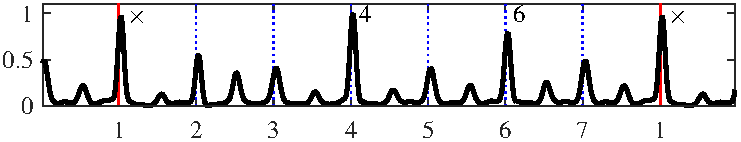
\includegraphics[width=\textwidth]{talaPatts/CMDf-mishraChapu-all-hi250-superflux-mvavg-normZ.pdf}} \\ \vspace{-1.35cm}
\subfloat[]{\label{fig:tt:CMDf:mishraChapu:lo}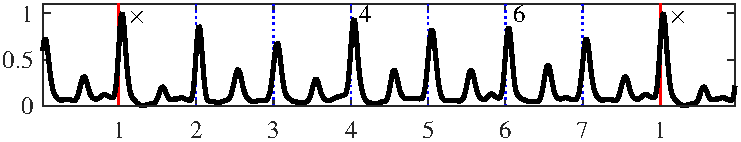
\includegraphics[width=\textwidth]{talaPatts/CMDf-mishraChapu-all-lo230-superflux-mvavg-normZ.pdf}}
\caption[Rhythm patterns in \gls{mishra chapu} \gls{tala} learned from \acrshort{CMDf} dataset]{Cycle length rhythmic patterns learned from \acrshort{CMDf} dataset for \gls{mishra chapu} \gls{tala}.}\label{fig:tt:CMDf:mishraChapu}
\end{figure}
%
%
% Tala pattern: CMD-mishraChapu-all-lo230-superflux-mvavg-normZ, CMD-mishraChapu-all-hi250-superflux-mvavg-normZ
\begin{figure}[t]
\captionsetup[subfigure]{labelformat=empty}
\centering
\subfloat[]{\label{fig:tt:CMD:mishraChapu:hi}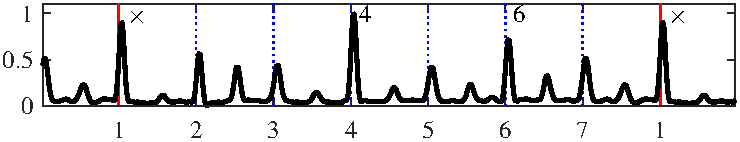
\includegraphics[width=\textwidth]{talaPatts/CMD-mishraChapu-all-hi250-superflux-mvavg-normZ.pdf}} \\ \vspace{-1.35cm}
\subfloat[]{\label{fig:tt:CMD:mishraChapu:lo}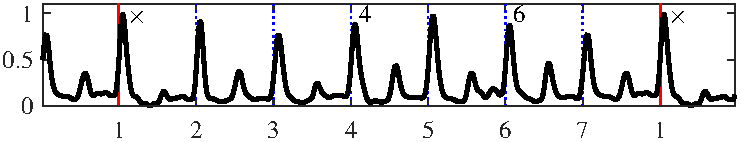
\includegraphics[width=\textwidth]{talaPatts/CMD-mishraChapu-all-lo230-superflux-mvavg-normZ.pdf}}
\caption[Rhythm patterns in \gls{mishra chapu} \gls{tala} learned from \acrshort{CMDs} dataset]{Cycle length rhythmic patterns learned from \acrshort{CMDs} dataset for \gls{mishra chapu} \gls{tala}.}\label{fig:tt:CMD:mishraChapu}
\end{figure}
%

The \figrefs{fig:tt:CMDf:rupaka}{fig:tt:CMD:rupaka}\ show the rhythm patterns for \gls{rupaka} \gls{tala}. Apart from the three level hierarachy of accents that is quite apparent, the half beat accent between the beats 2 and 3 are strong - indicating the often played 6+6 \gls{akshara} grouping structure of \gls{rupaka}, with a ternary meter.

The \figrefs{fig:tt:CMDf:mishraChapu}{fig:tt:CMD:mishraChapu}\ show the rhythm patterns for \gls{mishra chapu} \gls{tala}. We see that the \gls{anga} boundaries have strong left and right accents showing their use as anchor points to indicate the progression through the cycle. Though defined with a 3+2+2 \gls{akshara} grouping structure, a 1+2+2+2 structure is often seen in \gls{mishra chapu} \gls{tala}, which can be observed here, based on the strong left accent on beat 2. A additional strong left accent on beat 5 shows that it is also used as an anchor. 
%
% Tala pattern: CMDf-khandaChapu-all-lo230-superflux-mvavg-normZ, CMDf-khandaChapu-all-hi250-superflux-mvavg-normZ
\begin{figure}[t]
\captionsetup[subfigure]{labelformat=empty}
\centering
\subfloat[]{\label{fig:tt:CMDf:khandaChapu:hi}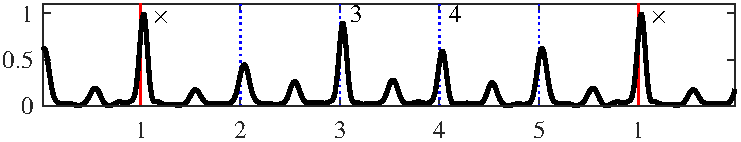
\includegraphics[width=\textwidth]{talaPatts/CMDf-khandaChapu-all-hi250-superflux-mvavg-normZ.pdf}} \\ \vspace{-1.35cm}
\subfloat[]{\label{fig:tt:CMDf:khandaChapu:lo}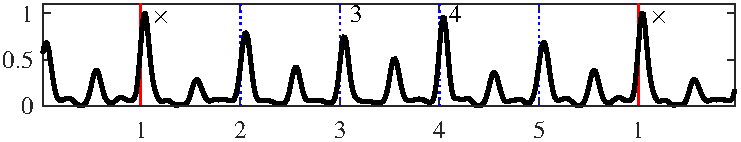
\includegraphics[width=\textwidth]{talaPatts/CMDf-khandaChapu-all-lo230-superflux-mvavg-normZ.pdf}}
\caption[Rhythm patterns in \gls{khanda chapu} \gls{tala} learned from \acrshort{CMDf} dataset]{Cycle length rhythmic patterns learned from \acrshort{CMDf} dataset for \gls{khanda chapu} \gls{tala}.}\label{fig:tt:CMDf:khandaChapu}
\end{figure}
%
%
% Tala pattern: CMD-khandaChapu-all-lo230-superflux-mvavg-normZ, CMD-khandaChapu-all-hi250-superflux-mvavg-normZ
\begin{figure}[t]
\captionsetup[subfigure]{labelformat=empty}
\centering
\subfloat[]{\label{fig:tt:CMD:khandaChapu:hi}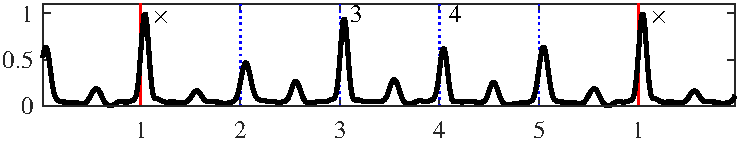
\includegraphics[width=\textwidth]{talaPatts/CMD-khandaChapu-all-hi250-superflux-mvavg-normZ.pdf}} \\ \vspace{-1.35cm}
\subfloat[]{\label{fig:tt:CMD:khandaChapu:lo}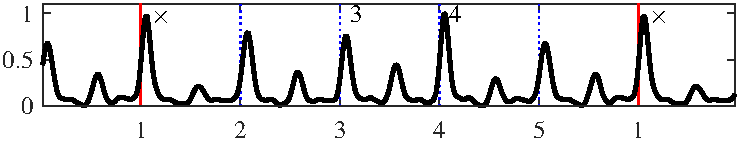
\includegraphics[width=\textwidth]{talaPatts/CMD-khandaChapu-all-lo230-superflux-mvavg-normZ.pdf}}
\caption[Rhythm patterns in \gls{khanda chapu} \gls{tala} learned from \acrshort{CMDs} dataset]{Cycle length rhythmic patterns learned from \acrshort{CMDs} dataset for \gls{khanda chapu} \gls{tala}.}\label{fig:tt:CMD:khandaChapu}
\end{figure}

The rhythm patterns of \gls{khanda chapu} \gls{tala} shown in \figrefs{fig:tt:CMDf:khandaChapu}{fig:tt:CMD:khandaChapu}\ have a strong left accent on beat 4, which is used an anchor within the cycle. A stronger right accent on beat 3 shows the progression through the unequal \glspl{anga}. The 2+1+2 \gls{akshara} grouping structure of \gls{khanda chapu} is often played out as 3+2 or 2+3, showing strong accents on beats 3 and 4. 

These are some observations from rhythm patterns that have interesting musicological significance. A professional Carnatic musician has informally validated these observations, but they still have to be formally studied in depth to make valid musicological conclusions. 
% An example of a corpus study with the dataset is an analysis of rhythmic patterns that occur in the dataset to see what musicological inferences can be made out of the analysis. We wish to independently verify 
% Statistical analysis of patterns in the dataset and what musicological inferences it can give out. 
%
%
%
% The bottom/top pane corresponds to the low/high frequency bands, respectively. The abscissa is the beat number within the cycle (dotted lines), with 1 indicating the \gls{sama} (marked with a red line). The start of each \gls{anga} is indicated with beat numbers at the top of each pane (\gls{sama} shown as $\times$).